\documentclass[10pt,twocolumn,letterpaper]{article}

\usepackage{iccv}
\usepackage{times}
\usepackage{epsfig}
\usepackage{graphicx}
\usepackage{amsmath}
\usepackage{amssymb}

% Include other packages here, before hyperref.
%%%%% NEW MATH DEFINITIONS %%%%%

\usepackage{amsmath,amsfonts,bm}

% Mark sections of captions for referring to divisions of figures
\newcommand{\figleft}{{\em (Left)}}
\newcommand{\figcenter}{{\em (Center)}}
\newcommand{\figright}{{\em (Right)}}
\newcommand{\figtop}{{\em (Top)}}
\newcommand{\figbottom}{{\em (Bottom)}}
\newcommand{\captiona}{{\em (a)}}
\newcommand{\captionb}{{\em (b)}}
\newcommand{\captionc}{{\em (c)}}
\newcommand{\captiond}{{\em (d)}}

% Highlight a newly defined term
\newcommand{\newterm}[1]{{\bf #1}}


% Figure reference, lower-case.
% \def\figref#1{figure~\ref{#1}}
% Figure reference, capital. For start of sentence
\def\Figref#1{Figure~\ref{#1}}
\def\twofigref#1#2{figures \ref{#1} and \ref{#2}}
\def\quadfigref#1#2#3#4{figures \ref{#1}, \ref{#2}, \ref{#3} and \ref{#4}}
% Section reference, lower-case.
% \def\secref#1{section~\ref{#1}}
% Section reference, capital.
\def\Secref#1{Section~\ref{#1}}
% Reference to two sections.
\def\twosecrefs#1#2{sections \ref{#1} and \ref{#2}}
% Reference to three sections.
\def\secrefs#1#2#3{sections \ref{#1}, \ref{#2} and \ref{#3}}
% Reference to an equation, lower-case.
\def\eqref#1{equation~\ref{#1}}
% Reference to an equation, upper case
\def\Eqref#1{Equation~\ref{#1}}
% A raw reference to an equation---avoid using if possible
\def\plaineqref#1{\ref{#1}}
% Reference to a chapter, lower-case.
\def\chapref#1{chapter~\ref{#1}}
% Reference to an equation, upper case.
\def\Chapref#1{Chapter~\ref{#1}}
% Reference to a range of chapters
\def\rangechapref#1#2{chapters\ref{#1}--\ref{#2}}
% Reference to an algorithm, lower-case.
\def\algref#1{algorithm~\ref{#1}}
% Reference to an algorithm, upper case.
\def\Algref#1{Algorithm~\ref{#1}}
\def\twoalgref#1#2{algorithms \ref{#1} and \ref{#2}}
\def\Twoalgref#1#2{Algorithms \ref{#1} and \ref{#2}}
% Reference to a part, lower case
\def\partref#1{part~\ref{#1}}
% Reference to a part, upper case
\def\Partref#1{Part~\ref{#1}}
\def\twopartref#1#2{parts \ref{#1} and \ref{#2}}

\def\ceil#1{\lceil #1 \rceil}
\def\floor#1{\lfloor #1 \rfloor}
\def\1{\bm{1}}
\newcommand{\train}{\mathcal{D}}
\newcommand{\valid}{\mathcal{D_{\mathrm{valid}}}}
\newcommand{\test}{\mathcal{D_{\mathrm{test}}}}

\def\eps{{\epsilon}}


% Random variables
\def\reta{{\textnormal{$\eta$}}}
\def\ra{{\textnormal{a}}}
\def\rb{{\textnormal{b}}}
\def\rc{{\textnormal{c}}}
\def\rd{{\textnormal{d}}}
\def\re{{\textnormal{e}}}
\def\rf{{\textnormal{f}}}
\def\rg{{\textnormal{g}}}
\def\rh{{\textnormal{h}}}
\def\ri{{\textnormal{i}}}
\def\rj{{\textnormal{j}}}
\def\rk{{\textnormal{k}}}
\def\rl{{\textnormal{l}}}
% rm is already a command, just don't name any random variables m
\def\rn{{\textnormal{n}}}
\def\ro{{\textnormal{o}}}
\def\rp{{\textnormal{p}}}
\def\rq{{\textnormal{q}}}
\def\rr{{\textnormal{r}}}
\def\rs{{\textnormal{s}}}
\def\rt{{\textnormal{t}}}
\def\ru{{\textnormal{u}}}
\def\rv{{\textnormal{v}}}
\def\rw{{\textnormal{w}}}
\def\rx{{\textnormal{x}}}
\def\ry{{\textnormal{y}}}
\def\rz{{\textnormal{z}}}

% Random vectors
\def\rvepsilon{{\mathbf{\epsilon}}}
\def\rvtheta{{\mathbf{\theta}}}
\def\rva{{\mathbf{a}}}
\def\rvb{{\mathbf{b}}}
\def\rvc{{\mathbf{c}}}
\def\rvd{{\mathbf{d}}}
\def\rve{{\mathbf{e}}}
\def\rvf{{\mathbf{f}}}
\def\rvg{{\mathbf{g}}}
\def\rvh{{\mathbf{h}}}
\def\rvu{{\mathbf{i}}}
\def\rvj{{\mathbf{j}}}
\def\rvk{{\mathbf{k}}}
\def\rvl{{\mathbf{l}}}
\def\rvm{{\mathbf{m}}}
\def\rvn{{\mathbf{n}}}
\def\rvo{{\mathbf{o}}}
\def\rvp{{\mathbf{p}}}
\def\rvq{{\mathbf{q}}}
\def\rvr{{\mathbf{r}}}
\def\rvs{{\mathbf{s}}}
\def\rvt{{\mathbf{t}}}
\def\rvu{{\mathbf{u}}}
\def\rvv{{\mathbf{v}}}
\def\rvw{{\mathbf{w}}}
\def\rvx{{\mathbf{x}}}
\def\rvy{{\mathbf{y}}}
\def\rvz{{\mathbf{z}}}

% Elements of random vectors
\def\erva{{\textnormal{a}}}
\def\ervb{{\textnormal{b}}}
\def\ervc{{\textnormal{c}}}
\def\ervd{{\textnormal{d}}}
\def\erve{{\textnormal{e}}}
\def\ervf{{\textnormal{f}}}
\def\ervg{{\textnormal{g}}}
\def\ervh{{\textnormal{h}}}
\def\ervi{{\textnormal{i}}}
\def\ervj{{\textnormal{j}}}
\def\ervk{{\textnormal{k}}}
\def\ervl{{\textnormal{l}}}
\def\ervm{{\textnormal{m}}}
\def\ervn{{\textnormal{n}}}
\def\ervo{{\textnormal{o}}}
\def\ervp{{\textnormal{p}}}
\def\ervq{{\textnormal{q}}}
\def\ervr{{\textnormal{r}}}
\def\ervs{{\textnormal{s}}}
\def\ervt{{\textnormal{t}}}
\def\ervu{{\textnormal{u}}}
\def\ervv{{\textnormal{v}}}
\def\ervw{{\textnormal{w}}}
\def\ervx{{\textnormal{x}}}
\def\ervy{{\textnormal{y}}}
\def\ervz{{\textnormal{z}}}

% Random matrices
\def\rmA{{\mathbf{A}}}
\def\rmB{{\mathbf{B}}}
\def\rmC{{\mathbf{C}}}
\def\rmD{{\mathbf{D}}}
\def\rmE{{\mathbf{E}}}
\def\rmF{{\mathbf{F}}}
\def\rmG{{\mathbf{G}}}
\def\rmH{{\mathbf{H}}}
\def\rmI{{\mathbf{I}}}
\def\rmJ{{\mathbf{J}}}
\def\rmK{{\mathbf{K}}}
\def\rmL{{\mathbf{L}}}
\def\rmM{{\mathbf{M}}}
\def\rmN{{\mathbf{N}}}
\def\rmO{{\mathbf{O}}}
\def\rmP{{\mathbf{P}}}
\def\rmQ{{\mathbf{Q}}}
\def\rmR{{\mathbf{R}}}
\def\rmS{{\mathbf{S}}}
\def\rmT{{\mathbf{T}}}
\def\rmU{{\mathbf{U}}}
\def\rmV{{\mathbf{V}}}
\def\rmW{{\mathbf{W}}}
\def\rmX{{\mathbf{X}}}
\def\rmY{{\mathbf{Y}}}
\def\rmZ{{\mathbf{Z}}}

% Elements of random matrices
\def\ermA{{\textnormal{A}}}
\def\ermB{{\textnormal{B}}}
\def\ermC{{\textnormal{C}}}
\def\ermD{{\textnormal{D}}}
\def\ermE{{\textnormal{E}}}
\def\ermF{{\textnormal{F}}}
\def\ermG{{\textnormal{G}}}
\def\ermH{{\textnormal{H}}}
\def\ermI{{\textnormal{I}}}
\def\ermJ{{\textnormal{J}}}
\def\ermK{{\textnormal{K}}}
\def\ermL{{\textnormal{L}}}
\def\ermM{{\textnormal{M}}}
\def\ermN{{\textnormal{N}}}
\def\ermO{{\textnormal{O}}}
\def\ermP{{\textnormal{P}}}
\def\ermQ{{\textnormal{Q}}}
\def\ermR{{\textnormal{R}}}
\def\ermS{{\textnormal{S}}}
\def\ermT{{\textnormal{T}}}
\def\ermU{{\textnormal{U}}}
\def\ermV{{\textnormal{V}}}
\def\ermW{{\textnormal{W}}}
\def\ermX{{\textnormal{X}}}
\def\ermY{{\textnormal{Y}}}
\def\ermZ{{\textnormal{Z}}}

% Vectors
\def\vzero{{\bm{0}}}
\def\vone{{\bm{1}}}
\def\vmu{{\bm{\mu}}}
\def\vtheta{{\bm{\theta}}}
\def\va{{\bm{a}}}
\def\vb{{\bm{b}}}
\def\vc{{\bm{c}}}
\def\vd{{\bm{d}}}
\def\ve{{\bm{e}}}
\def\vf{{\bm{f}}}
\def\vg{{\bm{g}}}
\def\vh{{\bm{h}}}
\def\vi{{\bm{i}}}
\def\vj{{\bm{j}}}
\def\vk{{\bm{k}}}
\def\vl{{\bm{l}}}
\def\vm{{\bm{m}}}
\def\vn{{\bm{n}}}
\def\vo{{\bm{o}}}
\def\vp{{\bm{p}}}
\def\vq{{\bm{q}}}
\def\vr{{\bm{r}}}
\def\vs{{\bm{s}}}
\def\vt{{\bm{t}}}
\def\vu{{\bm{u}}}
\def\vv{{\bm{v}}}
\def\vw{{\bm{w}}}
\def\vx{{\bm{x}}}
\def\vy{{\bm{y}}}
\def\vz{{\bm{z}}}

% Elements of vectors
\def\evalpha{{\alpha}}
\def\evbeta{{\beta}}
\def\evepsilon{{\epsilon}}
\def\evlambda{{\lambda}}
\def\evomega{{\omega}}
\def\evmu{{\mu}}
\def\evpsi{{\psi}}
\def\evsigma{{\sigma}}
\def\evtheta{{\theta}}
\def\eva{{a}}
\def\evb{{b}}
\def\evc{{c}}
\def\evd{{d}}
\def\eve{{e}}
\def\evf{{f}}
\def\evg{{g}}
\def\evh{{h}}
\def\evi{{i}}
\def\evj{{j}}
\def\evk{{k}}
\def\evl{{l}}
\def\evm{{m}}
\def\evn{{n}}
\def\evo{{o}}
\def\evp{{p}}
\def\evq{{q}}
\def\evr{{r}}
\def\evs{{s}}
\def\evt{{t}}
\def\evu{{u}}
\def\evv{{v}}
\def\evw{{w}}
\def\evx{{x}}
\def\evy{{y}}
\def\evz{{z}}

% Matrix
\def\mA{{\bm{A}}}
\def\mB{{\bm{B}}}
\def\mC{{\bm{C}}}
\def\mD{{\bm{D}}}
\def\mE{{\bm{E}}}
\def\mF{{\bm{F}}}
\def\mG{{\bm{G}}}
\def\mH{{\bm{H}}}
\def\mI{{\bm{I}}}
\def\mJ{{\bm{J}}}
\def\mK{{\bm{K}}}
\def\mL{{\bm{L}}}
\def\mM{{\bm{M}}}
\def\mN{{\bm{N}}}
\def\mO{{\bm{O}}}
\def\mP{{\bm{P}}}
\def\mQ{{\bm{Q}}}
\def\mR{{\bm{R}}}
\def\mS{{\bm{S}}}
\def\mT{{\bm{T}}}
\def\mU{{\bm{U}}}
\def\mV{{\bm{V}}}
\def\mW{{\bm{W}}}
\def\mX{{\bm{X}}}
\def\mY{{\bm{Y}}}
\def\mZ{{\bm{Z}}}
\def\mBeta{{\bm{\beta}}}
\def\mPhi{{\bm{\Phi}}}
\def\mLambda{{\bm{\Lambda}}}
\def\mSigma{{\bm{\Sigma}}}

% Tensor
\DeclareMathAlphabet{\mathsfit}{\encodingdefault}{\sfdefault}{m}{sl}
\SetMathAlphabet{\mathsfit}{bold}{\encodingdefault}{\sfdefault}{bx}{n}
\newcommand{\tens}[1]{\bm{\mathsfit{#1}}}
\def\tA{{\tens{A}}}
\def\tB{{\tens{B}}}
\def\tC{{\tens{C}}}
\def\tD{{\tens{D}}}
\def\tE{{\tens{E}}}
\def\tF{{\tens{F}}}
\def\tG{{\tens{G}}}
\def\tH{{\tens{H}}}
\def\tI{{\tens{I}}}
\def\tJ{{\tens{J}}}
\def\tK{{\tens{K}}}
\def\tL{{\tens{L}}}
\def\tM{{\tens{M}}}
\def\tN{{\tens{N}}}
\def\tO{{\tens{O}}}
\def\tP{{\tens{P}}}
\def\tQ{{\tens{Q}}}
\def\tR{{\tens{R}}}
\def\tS{{\tens{S}}}
\def\tT{{\tens{T}}}
\def\tU{{\tens{U}}}
\def\tV{{\tens{V}}}
\def\tW{{\tens{W}}}
\def\tX{{\tens{X}}}
\def\tY{{\tens{Y}}}
\def\tZ{{\tens{Z}}}


% Graph
\def\gA{{\mathcal{A}}}
\def\gB{{\mathcal{B}}}
\def\gC{{\mathcal{C}}}
\def\gD{{\mathcal{D}}}
\def\gE{{\mathcal{E}}}
\def\gF{{\mathcal{F}}}
\def\gG{{\mathcal{G}}}
\def\gH{{\mathcal{H}}}
\def\gI{{\mathcal{I}}}
\def\gJ{{\mathcal{J}}}
\def\gK{{\mathcal{K}}}
\def\gL{{\mathcal{L}}}
\def\gM{{\mathcal{M}}}
\def\gN{{\mathcal{N}}}
\def\gO{{\mathcal{O}}}
\def\gP{{\mathcal{P}}}
\def\gQ{{\mathcal{Q}}}
\def\gR{{\mathcal{R}}}
\def\gS{{\mathcal{S}}}
\def\gT{{\mathcal{T}}}
\def\gU{{\mathcal{U}}}
\def\gV{{\mathcal{V}}}
\def\gW{{\mathcal{W}}}
\def\gX{{\mathcal{X}}}
\def\gY{{\mathcal{Y}}}
\def\gZ{{\mathcal{Z}}}

% Sets
\def\sA{{\mathbb{A}}}
\def\sB{{\mathbb{B}}}
\def\sC{{\mathbb{C}}}
\def\sD{{\mathbb{D}}}
% Don't use a set called E, because this would be the same as our symbol
% for expectation.
\def\sF{{\mathbb{F}}}
\def\sG{{\mathbb{G}}}
\def\sH{{\mathbb{H}}}
\def\sI{{\mathbb{I}}}
\def\sJ{{\mathbb{J}}}
\def\sK{{\mathbb{K}}}
\def\sL{{\mathbb{L}}}
\def\sM{{\mathbb{M}}}
\def\sN{{\mathbb{N}}}
\def\sO{{\mathbb{O}}}
\def\sP{{\mathbb{P}}}
\def\sQ{{\mathbb{Q}}}
\def\sR{{\mathbb{R}}}
\def\sS{{\mathbb{S}}}
\def\sT{{\mathbb{T}}}
\def\sU{{\mathbb{U}}}
\def\sV{{\mathbb{V}}}
\def\sW{{\mathbb{W}}}
\def\sX{{\mathbb{X}}}
\def\sY{{\mathbb{Y}}}
\def\sZ{{\mathbb{Z}}}

% Entries of a matrix
\def\emLambda{{\Lambda}}
\def\emA{{A}}
\def\emB{{B}}
\def\emC{{C}}
\def\emD{{D}}
\def\emE{{E}}
\def\emF{{F}}
\def\emG{{G}}
\def\emH{{H}}
\def\emI{{I}}
\def\emJ{{J}}
\def\emK{{K}}
\def\emL{{L}}
\def\emM{{M}}
\def\emN{{N}}
\def\emO{{O}}
\def\emP{{P}}
\def\emQ{{Q}}
\def\emR{{R}}
\def\emS{{S}}
\def\emT{{T}}
\def\emU{{U}}
\def\emV{{V}}
\def\emW{{W}}
\def\emX{{X}}
\def\emY{{Y}}
\def\emZ{{Z}}
\def\emSigma{{\Sigma}}

% entries of a tensor
% Same font as tensor, without \bm wrapper
\newcommand{\etens}[1]{\mathsfit{#1}}
\def\etLambda{{\etens{\Lambda}}}
\def\etA{{\etens{A}}}
\def\etB{{\etens{B}}}
\def\etC{{\etens{C}}}
\def\etD{{\etens{D}}}
\def\etE{{\etens{E}}}
\def\etF{{\etens{F}}}
\def\etG{{\etens{G}}}
\def\etH{{\etens{H}}}
\def\etI{{\etens{I}}}
\def\etJ{{\etens{J}}}
\def\etK{{\etens{K}}}
\def\etL{{\etens{L}}}
\def\etM{{\etens{M}}}
\def\etN{{\etens{N}}}
\def\etO{{\etens{O}}}
\def\etP{{\etens{P}}}
\def\etQ{{\etens{Q}}}
\def\etR{{\etens{R}}}
\def\etS{{\etens{S}}}
\def\etT{{\etens{T}}}
\def\etU{{\etens{U}}}
\def\etV{{\etens{V}}}
\def\etW{{\etens{W}}}
\def\etX{{\etens{X}}}
\def\etY{{\etens{Y}}}
\def\etZ{{\etens{Z}}}

% The true underlying data generating distribution
\newcommand{\pdata}{p_{\rm{data}}}
% The empirical distribution defined by the training set
\newcommand{\ptrain}{\hat{p}_{\rm{data}}}
\newcommand{\Ptrain}{\hat{P}_{\rm{data}}}
% The model distribution
\newcommand{\pmodel}{p_{\rm{model}}}
\newcommand{\Pmodel}{P_{\rm{model}}}
\newcommand{\ptildemodel}{\tilde{p}_{\rm{model}}}
% Stochastic autoencoder distributions
\newcommand{\pencode}{p_{\rm{encoder}}}
\newcommand{\pdecode}{p_{\rm{decoder}}}
\newcommand{\precons}{p_{\rm{reconstruct}}}

\newcommand{\laplace}{\mathrm{Laplace}} % Laplace distribution

\newcommand{\E}{\mathbb{E}}
\newcommand{\Ls}{\mathcal{L}}
\newcommand{\R}{\mathbb{R}}
\newcommand{\emp}{\tilde{p}}
\newcommand{\lr}{\alpha}
\newcommand{\reg}{\lambda}
\newcommand{\rect}{\mathrm{rectifier}}
\newcommand{\softmax}{\mathrm{softmax}}
\newcommand{\sigmoid}{\sigma}
\newcommand{\softplus}{\zeta}
\newcommand{\KL}{D_{\mathrm{KL}}}
\newcommand{\Var}{\mathrm{Var}}
\newcommand{\standarderror}{\mathrm{SE}}
\newcommand{\Cov}{\mathrm{Cov}}
% Wolfram Mathworld says $L^2$ is for function spaces and $\ell^2$ is for vectors
% But then they seem to use $L^2$ for vectors throughout the site, and so does
% wikipedia.
\newcommand{\normlzero}{L^0}
\newcommand{\normlone}{L^1}
\newcommand{\normltwo}{L^2}
\newcommand{\normlp}{L^p}
\newcommand{\normmax}{L^\infty}

\newcommand{\parents}{Pa} % See usage in notation.tex. Chosen to match Daphne's book.

\DeclareMathOperator*{\argmax}{arg\,max}
\DeclareMathOperator*{\argmin}{arg\,min}

\DeclareMathOperator{\sign}{sign}
\DeclareMathOperator{\Tr}{Tr}
\let\ab\allowbreak

\usepackage[utf8]{inputenc} % allow utf-8 input
\usepackage[T1]{fontenc}    % use 8-bit T1 fonts
\usepackage{url}            % simple URL typesetting
\usepackage{booktabs}       % professional-quality tables
\usepackage{amsfonts}       % blackboard math symbols
\usepackage{nicefrac}       % compact symbols for 1/2, etc.
\usepackage{microtype}      % microtypography
\usepackage{multirow}
\usepackage{subfigure}
\usepackage{booktabs}
\usepackage{xcolor}
\usepackage{caption}
\usepackage{epsfig}
\usepackage{verbatim}
\usepackage{authorname}

% If you comment hyperref and then uncomment it, you should delete
% egpaper.aux before re-running latex.  (Or just hit 'q' on the first latex
% run, let it finish, and you should be clear).
\usepackage[pagebackref=true,breaklinks=true,letterpaper=true,colorlinks,bookmarks=false]{hyperref}

% \iccvfinalcopy % *** Uncomment this line for the final submission

\def\iccvPaperID{****} % *** Enter the ICCV Paper ID here
\def\httilde{\mbox{\tt\raisebox{-.5ex}{\symbol{126}}}}

% Pages are numbered in submission mode, and unnumbered in camera-ready
\ificcvfinal\pagestyle{empty}\fi

\begin{document}

%%%%%%%%% TITLE
\title{MeshMVS: Multi-View Stereo Guided Mesh Reconstruction}

\author{First Author\\
Institution1\\
Institution1 address\\
{\tt\small firstauthor@i1.org}
% For a paper whose authors are all at the same institution,
% omit the following lines up until the closing ``}''.
% Additional authors and addresses can be added with ``\and'',
% just like the second author.
% To save space, use either the email address or home page, not both
\and
Second Author\\
Institution2\\
First line of institution2 address\\
{\tt\small secondauthor@i2.org}
}

\maketitle
% Remove page # from the first page of camera-ready.
\ificcvfinal\thispagestyle{empty}\fi

\newcommand{\todo}[1]{{\textcolor{red}{\bf [#1]}}}
% \newcommand{\siyu}[1]{{\color{blue}[Siyu: #1]}}
% command for Siyu's comment is already in authorname.sty

\newcommand{\figref}[1]{Figure~\ref{fig:#1}}
\newcommand{\tabref}[1]{Table~\ref{tab:#1}}
\newcommand{\equref}[1]{Equation~(\ref{equ:#1})}
\newcommand{\secref}[1]{Section~\ref{sec:#1}}
\newcommand{\subsecref}[1]{Sub-section~\ref{subsec:#1}}
\newcommand{\tableref}[1]{Table~\ref{table:#1}}

%%%%%%%%% BODY TEXT
\begin{abstract}

    Deep learning based 3D shape generation methods generally utilize latent features extracted from color images to encode the objects' semantics and guide the shape generation process.
    These color image semantics only implicitly encode 3D information, potentially limiting the accuracy of the generated shapes.
    In this paper we propose a multi-view mesh generation method which incorporates geometry information in the color images explicitly by using the features from intermediate 2.5D depth representations of the input images and regularizing the 3D shapes against these depth images.
    Our system first predicts a coarse 3D volume from the color images by probabilistically merging voxel occupancy grids from individual views.
    Depth images corresponding to the multi-view color images are predicted which along with the rendered depth images of the coarse shape are used as a contrastive input whose features guide the refinement of the coarse shape through a series of graph convolution networks.
    Attention-based multi-view feature pooling is proposed to fuse the contrastive depth features from different viewpoints which are fed to the graph convolution networks.
    
    % Additional constrains between the rendered depths of the predicted shapes and the predicted depth maps are introduced to further regularize the shape generation process.
    % A series of graph convolution networks are applied to refine the shape in a coarse to fine manner all of which utilize contrastive depth input at the current stage of refinement.

    We validate the proposed multi-view mesh generation method on ShapeNet, where we obtain a significant improvement with 34\% decrease in chamfer distance to ground truth and 14\% increase in the F1-score compared with the state-of-the-art multi-view shape generation method.
    % \rakesh{chamfer distance current - 1.45 cm, pixel2mesh++- 2.2 cm (the unit of chamfer distance reported in the Pixel2Mesh(++) paper is m^2 * 1000, it might confuse the reviewers/readers if we report these numbers}
\end{abstract}

\siyu{We should re-summarize the main contributions of the proposed work. Some hints: 1. Extend mesh-rcnn from single view to multi-views which can obtain the initial mesh significantly superior to the state-of-the-art works (ellipsoid, single-view mesh-rcnn) (+10\%?+20\%?). 2. Introduce the contrastive feature extractor in GCNN which considers the reconstructed depth from MVS-Net and rendered depth from voxel grid, and further improve (+3.8\%) the quality of the mesh in the refinement module.}
\section{Introduction}

3D shape generation is a long-standing research problem in computer vision and computer graphics with applications in autonomous driving, augmented reality, etc. Conventional approaches mainly leverage multi-view geometry based on stereo correspondences between images but are restricted by the coverage provided by the input views. With the availability of large-scale 3D shape datasets and the success of deep learning in several computer vision tasks, 3D representations such as voxel grid~\cite{3dr2n2, tulsiani2017multi, yan2016perspective} and point cloud~\cite{yang2018foldingnet, fan2017point} have been explored for single-view 3D reconstruction.
Among them, triangle mesh representation has received the most attention as it has various desirable properties for a wide range of applications and is capable of modeling detailed geometry without high memory requirement.

Single-view 3D reconstruction methods~\cite{wang2018pixel2mesh,huang2015single,kar2015category,su2014estimating} generate the 3D shape from merely a single color image but suffer from limited visibility due to occlusion and high dependency on training views leading to weaker generalization to different input views, resulting in low quality reconstructions.
\siyu{What are the limitations of single-view approaches? Limited visibility, high dependency on prediction ability and weak generalization (domain transfer)... Need some discussion.}
\rakesh{Edited preceding sentence based on the comments}
% \rakesh{Implying that multi-view methods can generalize better than single-view to different domains/semantic categories during test time might be too strong of a claim, training on cars and testing on planes might be equally bad, whether it's single-view or multi-view}
Multi-view methods~\cite{wen2019pixel2mesh++,3dr2n2,kar2017lsm,mcrecon2017} extend the input to images from different viewpoints which provides more visual information and improves the accuracy of the generated shapes.
Recent work in multi-view mesh reconstruction~\cite{wen2019pixel2mesh++} introduces a multi-view deformation network using perceptual feature from each color image for refining the meshes generated by Pixel2Mesh~\cite{wang2018pixel2mesh}.
Although promising results were obtained, this method relies on perceptual features from color images which do not explicitly encode the objects' geometry and could restrict the accuracy of the 3D models.
The work is also constrained by the topology of the initial shape, an ellipsoid, which limits the accuracy of the shapes from subsequent refinement modules.
Furthermore, their use of multi-view information does not take into account phenomena such as occlusion and visibility.
\siyu{According to the main contributions of the proposed approach, we can discuss bout the limitations of the current multi-view approaches. First, the quality of the initial mesh is weak, and the initial topology it vital to the subsequent refinement module. Second, the refinement module is only image-based, without considering the 3D information (depth) or the information of multi-view constraints. After discussing about the existed problems, we can propose our solutions.}
\rakesh{Edits made}

% Inspired by the authors~\cite{yao2020front2back} demonstrate that using intermediate, image-centric 2.5D representations instead of directly generating 3D shapes in global frame raw from 2D images can improve 3D reconstruction quality.

% But their work relies on handcrafted heuristics for view interpolation and fuse 2.5D representations to 3D shapes using traditional, non-differentiable techniques~\cite{kazhdan2013screened}.
% Additionally Pixel2Mesh~\cite{wang2018pixel2mesh} and Pixel2Mesh++~\cite{wen2019pixel2mesh++} deform a fixed template mesh to obtain the desired shapes of all the objects which restricts the topology of the final output.

In this work, we present a novel multi-view mesh generation method where we start by predicting coarse volumetric occupancy grid representations of the color images.
Using this representation for further refinement rather than a predefined template shape allows us to generate shapes with more accurate topology~\cite{gkioxari2019meshrcnn}.
We then use Graph Convolutional Network (GCN)~\cite{scarselli2008graph,wang2018pixel2mesh} to fine-tune the volumetric representation to surface mesh in a coarse-to-fine manner.
The GCN obtains features of the graph nodes (mesh vertices) from contrastive depth features alongside the RGB perceptual features.
The contrastive depth features are extracted from the rendered depth maps of the intermediate shape and predicted depth maps from a multi-view stereo network.
Constrains between the rendered depths and predicted depths at different viewpoints are further added.
This allows our system to better reason about the transformation required to deform the intermediate shapes to confirm to the predictions by the multi-view stereo network.
We also propose an attention-based method to fuse features from multiple views that can learn the importance of different views for each of the mesh vertices allowing the system to reason about visibility and occlusion in different input views.
\siyu{The description of the proposed approaches in this paragraph is too concrete. Try to explain the intuition behind the corresponding methods and the problems they can solve.}
\rakesh{Edits made}
% \figref{system_architecture} depicts our system architecture.
% \rakesh{Note: There is no mesh upsampling between the GCNs in Mesh R-CNN based system}

We validate our method on the ShapeNet~\cite{chang2015shapenet} benchmark and our method achieves the best performance among all previous mesh generation methods, with 14\% increase in F1-score compared to the state-of-the-art.
\siyu{Give some explicit statistics demonstrating the performance of your proposed approach. For example, we achieve the best performance in aaa-benchmark, and +aa\%, +bb\% performance compared with the state-of-the-art.}
\rakesh{statistics added}

% lead to a

% which can be easily used to extend existing single-view 3D shape generation methods to multi-view versions.
% We start by estimating the depth maps of the multi-view RGB images using an extended MVSNet~\cite{yao2018mvsnet}. This is followed by a feature extraction network for obtaining high-level features from these depth images. An attention-based feature pooling aggregates the multi-view features which are then used by graph convolutional networks to deform an initial mesh to the final shape in a coarse-to-fine manner. We use a differentiable renderer on the predicted meshes (both intermediate and final) in order to obtain additional constraints on the deformation process in terms of the rendered depths.
% The depth predictions leverage geometry information directly into the deformation process while the multi-head attention mechanism acts as an effective method to fuse the geometric features from different views facilitating the mesh generation process to produce a finer output.


%%%%%%%%% Related works
\section{Related Work}
\siyu{I think the classification of related works in Pixel2Mesh++ is more reasonable, that is 3D shape representation, single-view shape generation, and multi-view shape generation.
The ``Traditional Shape Generation Methods'' can be merged into ``single-view shape generation'' and ``multi-view shape generation''. We donot have to survey ``Depth Estimation'', which seems irrelevant to our approach.}
\rakesh{
    Depth estimation survey removed.
    Added paragraph for 3D Shape representation
    Restructured the related work categories to single-view and multi-view methods
}

\paragraph{3D Shape Representation}
3D occupancy grid has been a popular representation since conventional CNNs can be used to generate them~\cite{3dr2n2,kar2017lsm}.
More recently, mesh representation is being increasingly used for 3D reconstruction~\cite{wang2018pixel2mesh,wen2019pixel2mesh++} where a template mesh (an ellipsoid) is deformed to obtain the final shape.
This approach struggles in reconstructing shapes whose topologies are very different from the template mesh.
\cite{gkioxari2019meshrcnn} proposes a hybrid approach where a coarse occupancy grid is first predicted from single image which is converted to mesh representation and further refined using mesh deformations.
We adopt a similar approach in our work where we predict the coarse occupancy grid from multi-view images which are used as the initial shape for succeeding refinements.
Other shape representations include point clouds~\cite{fan2017point,yang2018foldingnet,jia2020dv}, implicit surfaces~\cite{park2019deepsdf}, depth images~\cite{yao2018mvsnet,yao2019recurrent} etc.


\textcolor{Red}{
We can discuss about:
1. Different representations of 3D shape in learning-based approaches. Please refer to the survey in Pixel2Mesh++.
2. The existed works of initial mesh generation, and especially the limitations of such methods and the effect of initial mesh on the final results.
3. To overcome such limitations, we use the voxel grid as the 3D representation of the initial mesh, and multi-view ... to obtain the initial mesh.
\paragraph{Single-view Shape Generation.}
Point cloud, voxel grid and mesh... Maybe we can mainly focus on the voxel grid and mesh.
\paragraph{Multi-view Shape Generation.}
Mainly focus on the limitations of existed methods and how can we handle such limitations.
}

\begin{figure*}[t]
\begin{center}
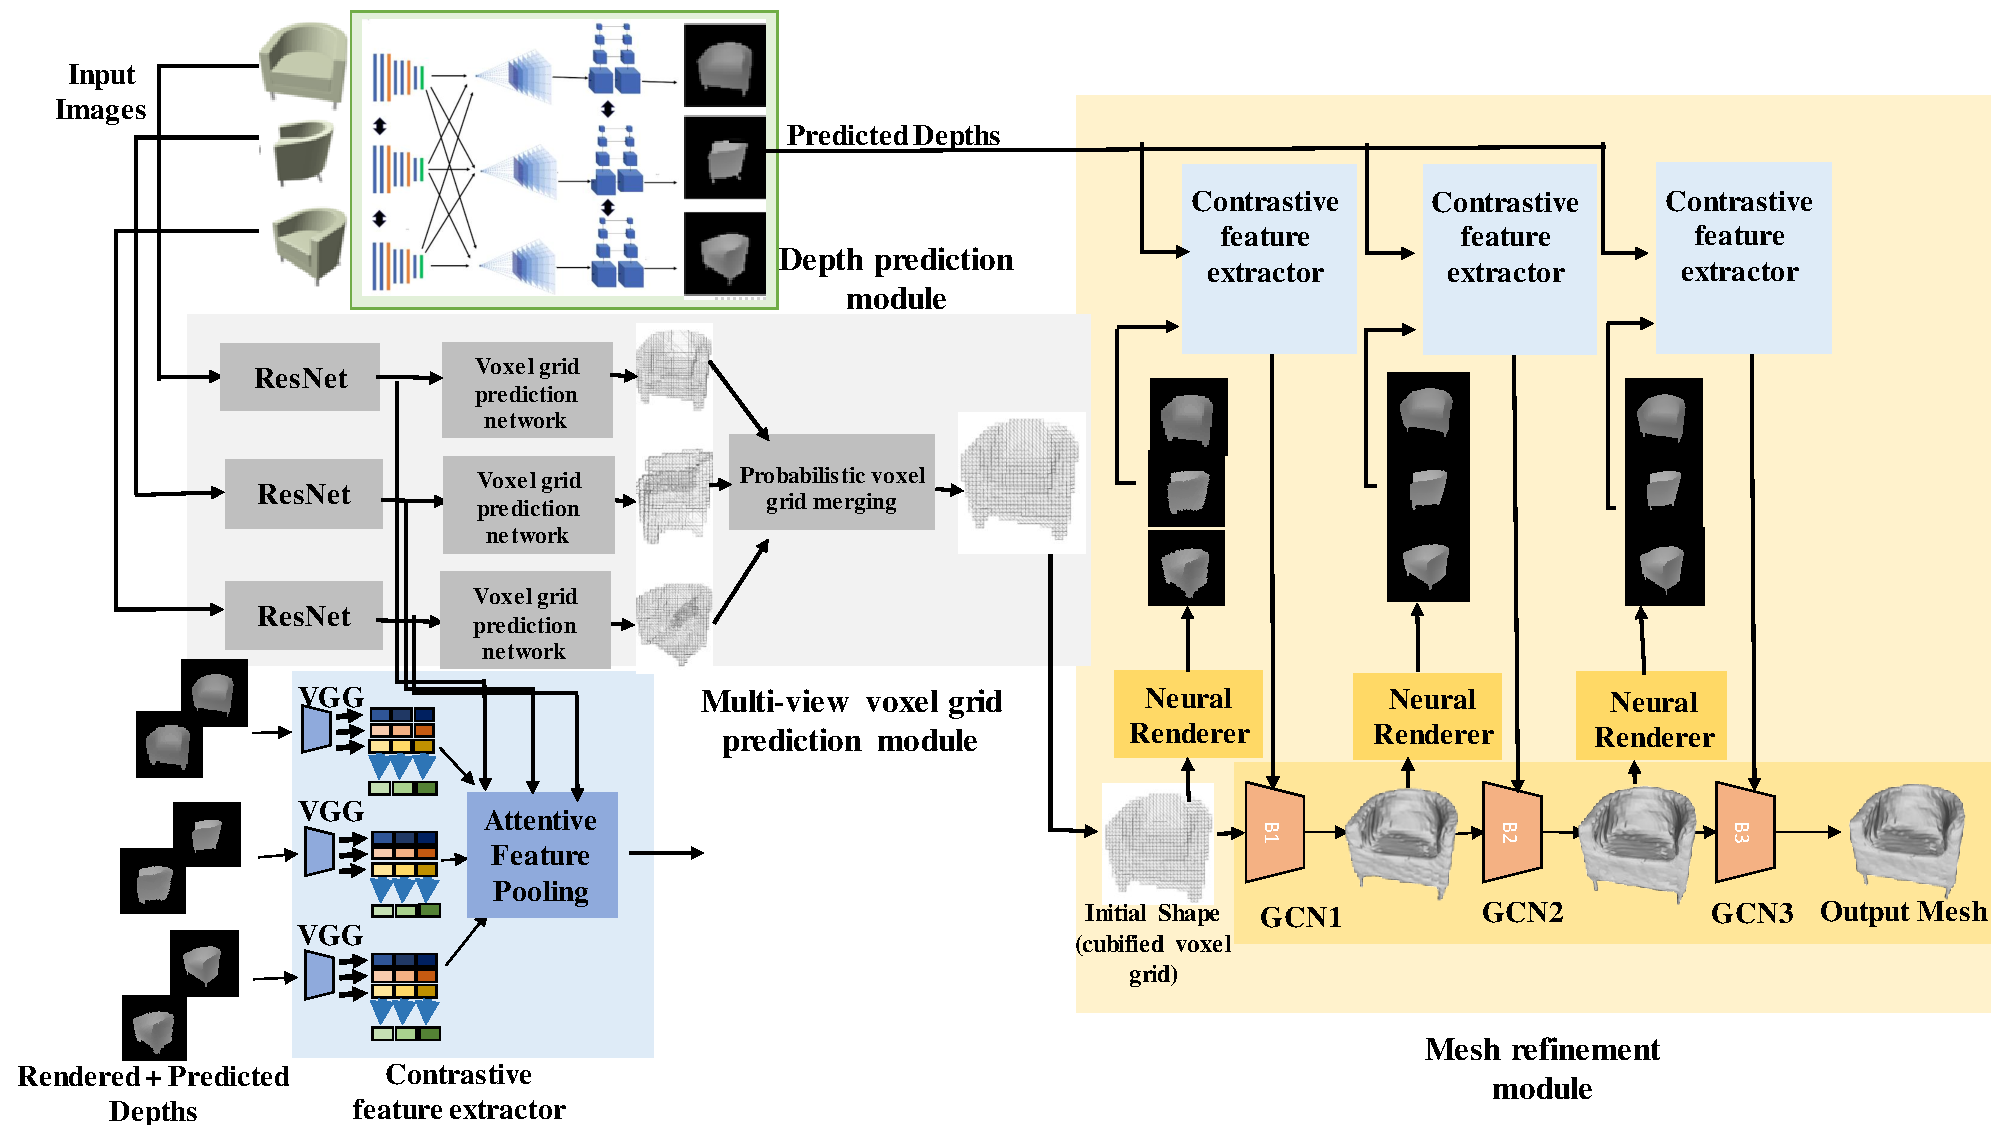
\includegraphics[width=\linewidth]{imgs/meshrcnn_architecture.pdf}
\end{center}
\caption{
    \textbf{Architecture of the proposed method}.
    The \emph{voxel grid prediction module} predicts coarse voxel grid representation by using CNN to predict voxel grids for each input image and then probabilistically merging them.
    A series of \emph{GCN}s further refine the cubified voxel grid in a coarse-to-fine manner
    using \emph{contrastive depth features} from rendered depths of the current shape and the predicted depths from \emph{depth prediction module} along with RGB image features.
    Multi-view features are pooled using a attention-based mechanism.
    \siyu{Replace this figure with a simplified one and add a long caption describing the whole framework.}
    \rakesh{simplified figure has been placed and caption has been expanded}
}
\label{fig:system_architecture}
\end{figure*}

\paragraph{Single-view Shape Generation.}
Traditional single-view shape generation methods like~\cite{durou2008numerical,zhang1999shape,favaro2005geometric} reason about shading, texture and defocus to reason about visible parts of the object and infer its 3D geometry.
Earlier learning-based approaches~\cite{huang2015single, su2014estimating} use shape component retrieval and deformation from a large dataset for single-view 3D shape generation.
\cite{kurenkov2018deformnet} extend this idea by introducing free-form deformation networks on retrieved object templates from a database.
Some work learn shape deformation from ground truth foreground masks of 2D images~\cite{kar2015category,yan2016perspective,tulsiani2017multi}.
\cite{3dr2n2,hane2017hierarchical,johnston2017scaling} can learning 3D volumetric representations through deep learning.
Predicting 3D mesh from single-view color images has been proposed in~\cite{wang2018pixel2mesh,pan2019deep,gkioxari2019meshrcnn, tang2019skeleton}.
DR-KFS~\cite{jin2019drkfs} introduces a differentiable visual similarity metric to learn single-view 3D shape generation
while SeqXY2SeqZ~\cite{han2020seqxy2seqz} represents 3D shapes using a set of 2D voxel tubes for shape reconstruction.
Front2Back~\cite{yao2020front2back} generates 3D shapes by fusing predicted depth and normal images and
DV-Net~\cite{jia2020dv} predicts dense object point clouds using dual-view RGB images with a gated control network to fuse point clouds from the two views.
FoldingNet~\cite{yang2018foldingnet} learns to reconstruct arbitrary point clouds from a single 2D grid.
AtlasNet~\cite{groueix2018papier} use learned parametric representation
while \cite{mescheder2019occupancy,park2019deepsdf,liu2019learning,liu2019dist,murez2020atlas} employ implicit surface representation to reconstruct 3D shapes.

\paragraph{Multi-view Shape Generation.}
Multi-view 3D model generation has traditionally been tackled using stereo geometry principles.
Among them, structure-from-motion (SfM)~\cite{schonberger2016structure,agarwal2011building,cui2015global,cui2017hsfm} and simultaneous localization and mapping (SLAM)~\cite{cadena2016pastslam,mur2015orb,engel2014lsd,whelan2015elasticfusion} are popular techniques that perform 3D reconstruction and camera pose estimation at the same time.
% Closer to our problem setup, multi-view stereo methods infer 3D geometry from images with known camera parameters.
% These generally fall into one of two categories: Volumetric and Point Cloud based methods.
Similarly, traditional multi-view stereo methods infer 3D geometry from images with known camera parameters either using
volumetric representation~\cite{kutulakos2000theory, seitz1999photorealistic} or
point cloud representation~\cite{furukawa2009accurate, lhuillier2005quasi}.
These methods extract local image features, match them across images and use the matches to estimate 3D geometry.
While the results of these works are impressive in terms of quality and completeness of reconstruction, they still struggle with poorly textured and reflective surfaces and require carefully selected input views.

Deep learning based approaches can learn to infer 3D structure from training data and can be robust against poorly textured and reflective surfaces as well as limited and arbitrarily selected input views.
\cite{hartmann2017learned_16,deepmvs2018,yao2018mvsnet,chen2019point,luo2019pmvsnet,gu2019cascade,yao2019recurrent} propose multi-view stereo models from learned cost volumes to predict depth images.
Recurrent Neural Networks (RNN) based methods~\cite{3dr2n2, kar2017lsm, mcrecon2017} are another popular solution to solve this problem.
\cite{mcrecon2017, lin2019photometric} introduce image silhouettes along with adversarial multi-view constraints and optimize object mesh models using multi-view photometric constraints.
Pixel2Mesh++~\cite{wen2019pixel2mesh++} extends single-view Pixel2Mesh~\cite{wang2018pixel2mesh} to multi-view image input by introducing cross-view perceptual feature pooling and multi-view deformation reasoning but struggles to reconstruct complex shape topologies due to its use of ellipsoidal template shape which it deforms to the final shape.
Our work avoids this pitfall by first predicting a coarse volumetric model which can represent complex topologies and then applying deformations on it to get a finer shape as the final model.

% Pixel2Mesh~\cite{wang2018pixel2mesh} utilizes a single image of an object to predict its triangle mesh using perceptual features extracted from the image as GCN input.
% Voxel2Mesh~\cite{wickramasinghe2019voxel2mesh} extends Pixel2Mesh by using 3D volumes as input instead of 2D images.
% Pan et al.~\cite{pan2019deep} propose a similar progressive framework which alternates between neural networks for mesh deformation and topology modification for pruning error-prone faces.
% DR-KFS~\cite{jin2019drkfs} introduces a differentiable visual similarity metric for improving reconstruction quality of various shape generation methods.
% SeqXY2SeqZ~\cite{han2020seqxy2seqz} represent 3D shapes using a set of 2D voxel tubes which are predicted using RNN with a single image as input.
% Front2Back~\cite{yao2020front2back} generate 3D shapes by fusing predicted depth and normal images using Screen Poisson surface reconstruction~\cite{kazhdan2013screened}.
% Mesh R-CNN~\cite{gkioxari2019meshrcnn} utilizes instance segmentation to predict a coarse voxel grid which is further refined using GCNs to obtain a mesh from a single image.
% \cite{tang2019skeleton} further break down shape generation into skeleton prediction followed by voxel grid generation and finally GCN based mesh refinement.

% Recurrent Neural Networks (RNN) have been a popular solution for multi-view 3D reconstruction.
% 3D-R2N2~\cite{3dr2n2} employs 3D RNN with encoder-decoder architecture
% while LSM~\cite{kar2017lsm} uses recurrent 3D features grid fusion to predict 3D occupancy grid models.
% Gwak et al.~\cite{mcrecon2017} use image silhouettes along with adversarial multi-view constraints to estimate 3D voxel grid models.
% \cite{lin2019photometric} optimizes object mesh models using multi-view photometric constraint by piecewise image alignment of each mesh faces' rasterized projections.
% Pixel2Mesh++~\cite{wen2019pixel2mesh++} uses feature statistics from multi-view images to refine the mesh generated by Pixel2Mesh by further deforming the mesh vertices within a local neighborhood.

% We refer our readers to a recent survey on Deep Geometry Learning ~\cite{xiao2020survey} for a more comprehensive review of the related work on this topic.

% \paragraph{Depth Estimation}
% Compared to 3D shape generation, depth prediction is an easier problem formulation since it simplifies the task to per-view depth map estimation.
% Traditional methods ~\cite{campbell2008using,galliani2015massively,schonberger2016pixelwise} use multi-view stereo principles for depth prediction.
% Deep learning based multi-view stereo depth estimation was first introduced in~\cite{hartmann2017learned_16} where a learned cost metric is used to estimate patch similarities.
% DeepMVS~\cite{deepmvs2018} warps multi-view images to 3D space and then applies deep networks for regularization and aggregation to estimate depth images.
% Learned 3D cost volume based depth prediction was proposed in MVSNet~\cite{yao2018mvsnet} where a 3 dimensional cost volume is built using homographically warped 2D features from multi-view images and 3D CNNs are used for cost regularization and depth regression.
% This idea was further extended by~\cite{chen2019point,luo2019pmvsnet, gu2019cascade,yao2019recurrent}.

% Our system aims to combine the strengths of GCN based methods and depth prediction methods to improve the accuracy of the 3D structure while still ensuring completeness.

%%%%%%%%% The Proposed Architecture
\section{Methodology}
\siyu{The current content of the ``Methodology'' section is too limited, try to expand this content.}

\figref{system_architecture} shows the architecture of the proposed system which takes as input multi-view color images of an object with known poses and outputs a triangle mesh representing the surface of the object.
\siyu{Before Section 3.1, at least two point should be mentioned: 1. The input and output of this approach, including some notations. 2. An overview of the whole methodology including some reference of the explicit sections. And it is also a hierarchical structure of the ``Methodology'' section.}

\subsection{Multi-view Voxel Grid Prediction}
\label{subsec:multiview_voxel}

\paragraph{Single-view Voxel Grid Prediction}
The single-view voxel branch consists of a ResNet feature extractor and a fully convolutional voxel grid prediction network. It generates the coarse initial shape of an object from one viewpoint as voxel occupancy grid using a color image. Here, we set the resolution of the generated voxel occupancy grid as 32 $\times$ 32 $\times$ 32. The voxel prediction networks for all viewpoints share the same weights.
% following Mesh R-CNN~\cite{gkioxari2019meshrcnn}.
\siyu{Should cite MeshRCNN reference here. As well, the implementation differences should be detailized here.}

\paragraph{Probabilistic Occupancy Grid Merging}
\siyu{Present a figure to demonstrate the ``probabilistic occupancy grid merging'', the intermediate results of this module.}
\siyu{This method is inspired by the traditional occupancy grid merging approaches in robotics? If so, try to cite the references and tell the differences between yours and the existed ones.}
Voxel occupancy grid predicted from a single viewpoint suffers from occlusion and limited visibility. In order to fuse voxel grids from different viewpoints, we propose a probabilistic occupancy grid merging method which merges the voxel grids from each input viewpoint probabilistically to obtain the final voxel grid output. This allows occluded regions in one view to be estimated from other views where those regions are visible as well as increase the confidence of prediction in overlapping regions.
Occupancy probability of each voxel is represented by $p(x)$ which is converted to log-odds (logit):
% \footnote{In practice the \emph{voxel branch} directly predicts the log-odds instead of probabilities}

\begin{equation}
    l(x) = log \frac{p(x)}{1 - p(x)}
    \label{equ:logodds}
\end{equation}

Bayesian update on the probabilities reduce to simple summation of log likelihoods~\cite{konolige1997improved}. Hence, the multi-view log-odds of a voxel is given by:

\begin{equation}
    l(x) = l_1(x) + l_2(x) + ... + l_n(x)
    \label{equ:logodds_sum}
\end{equation}

\noindent where $l_i$ is the voxel's log-odds in view $i$ and $n$ is the number of input views.
The final voxel probability $x$ is obtained by applying the inverse function of \equref{logodds} which is a sigmoid function.
% The final probability of the voxel $x$ can be obtained by applying the inverse function of \equref{logodds} which is a sigmoid function.

\siyu{We should add an experiment and study the effect of the quality of the initial mesh on the final mesh reconstruction results, including the ellipsoid, single-view MeshRCNN, our MeshRCNN with different number of views.}

\subsection{Mesh Refinement}
\siyu{Present a figure to explain the detailed mechanism of the mesh refinement module.}
The \texttt{cubified} mesh from the voxel branch only provides a coarse reconstruction of the object's surface. We apply graph convolutional networks which represent each mesh vertex as one graph node and deforms them to more accurate positions.

\paragraph{GCN-based Mesh Deformation}
\siyu{The intuition and basic operations of graph-cnn-based mesh deformation should be given first. Then, how does the previous approach obtain the features. Any limitations and problems of the previous approaches?}
The features pooled from multi-view images along with 3D coordinates of the vertices in world frame are used as features of the graph nodes.
Series of Graph-based Convolutional Network (GCN) blocks are applied to deform a mesh at the current stage to the next stage, starting with the \texttt{cubified} voxel grids.
A graph convolution deforms mesh vertices by propagating features from neighboring vertices by applying
$f_{i}^{'} = ReLU(W_0f_i + \sum_{j \in \mathcal{N}(i)} W_1 f_j)$ where $\mathcal{N}(i)$ is the set of neighboring vertices of the \emph{i}-th vertex in the mesh, $f_{\{\}}$ represents the feature vector of a vertex, and $W_0$ and $W_1$ are learnable parameters of the model.
Each GCN block utilizes several graph convolutions to transform the vertex features along with a final \emph{vertex refinement} operation where the features along with vertex coordinates are further transformed as $v_i^{'} = v_i + tanh(W_{vert}[f_i;v_i])$ where the matrix $W_{vert}$ is another learnable parameter to obtain the deformed mesh.

\label{subsec:contrastive_depth_feature_extraction}
\paragraph{Contrastive Depth Feature Extraction}
\siyu{Can you give a figure demonstrating the module of contrastive depth feature extraction? Since in Figure 1 of the ICLR submitted paper, you also input the RGBD feature maps from ResNet, do you still use it?}
\cite{yao2020front2back} demonstrate that using intermediate, image-centric 2.5D representations instead of directly generating 3D shapes in global frame from raw 2D images can improve 3D reconstruction quality.
We therefore propose to formulate the features for graph nodes using 2.5D depth maps as input additional inputs alongside the RGB features.
% and \zhiwen{todo} to contrast the depth map at current refinement stage against the predicted depths.
Specifically, we render the meshes at different GCN stages to depth image at all the input views using~\cite{kato2018renderer} and use them along with predicted depths for depth feature extraction. We call this form of depth input \texttt{contrastive depth} as it contrasts the rendered depths of the current mesh against the predicted depths and allows the network to reason about the deformation better than when using predicted depth or color images alone.
% construct the feature vector from semantic features of the input color images~\cite{wang2018pixel2mesh}, we formulate the input for feature extraction network using geometry representations.
% However, works similar to Pixel2Mesh~\cite{wang2018pixel2mesh} construct the feature vector from semantic features of the input color images. Here, we formulate the input for feature extraction network using geometry representations. Specifically, we render the meshes at different GCN stages to depth image at all the input views using~\cite{kato2018renderer} and augment them as additional inputs for depth feature extraction.
% We call this form of depth input \emph{contrastive depth} as it contrasts the rendered depths of the current mesh against the predicted depths and constrain the deformed mesh in a coarse-to-fine manner.
Given the 2D features, corresponding feature vectors of individual vertices can be found by projecting the 3D vertex coordinates to the feature planes using known camera parameters.
We use VGG-16~\cite{simonyan2014vgg} as our contrastive depth feature extraction network.
% Along with the contrastive depth features, we also use the RGB features from ResNet calculated for voxel branch as input for mesh deformation as well.

% and allows the network to reason about the deformation required better than when using predicted depths alone.
% Multiple methods for augmenting the two depths were tried among which using concatenated rendered and predicted depth as input for depth feature extraction gave the best result.
% Along with the contrastive depth features, we also use the RGB features from ResNet calculated for voxel branch as input for mesh deformation as well.

\label{subsec:depth_prediction}
\paragraph{Multi-View Depth Estimation}
\siyu{In order to explain how can we obtain the initial depth images as the input, this paragraph should be put in front of the ``Mesh Refinement'' section, or the front of the ``3. Methodology''. We donot have to mention the details of MVS-Net, while some implementation details, like the view selection mechanism, resolution, network structure design, any difference from the standard MVS-Net or Cas-MVSNet.}
We extend MVSNet~\cite{yao2018mvsnet} and predict the depth maps of all views since the original implementation predicts depth of only one reference view.
This is achieved by transforming the feature volumes to each view's coordinate frame using homography warping
and applying identical cost volume regularization and depth regression on each view.
Detailed network architecture diagram of this module is provided in the appendix.
\siyu{Do we have to add an experiment and compare the results give different settings of MVS-Net, such as the resolution of the depth images or we can add some noise to the depth. That is to study the effect of the quality of the depth on the final mesh reconstruction results and how sensitive is the refinement module to the depth quality.}

% which constructs a regularized 3D cost volumes
% to estimate the depth map of the reference view.
% Here, we extend MVSNet to predict the depth maps of all views instead of only the reference view.

% This allows the reuse of pre-regularization feature volumes for efficient multi-view depth prediction invariant to the order of input images.

\begin{figure*}[t]
\begin{center}
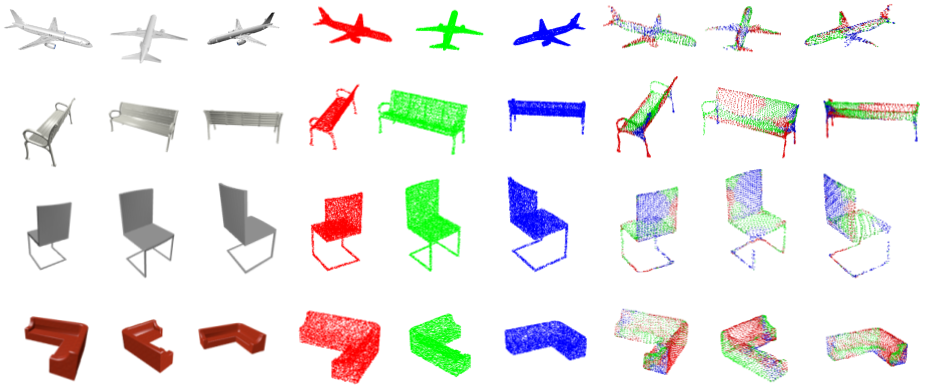
\includegraphics[width=\linewidth]{imgs/attention_weights_visualization.png}
\end{center}
    \caption{
        \textbf{Attention weights visualization.}
        From left to right: input images from 3 viewpoints, corresponding ground truth point clouds color-coded by their view order and the predicted mesh vertices color-coded by the attention weights of the views.
        Only the view with maximum attention weight is visualized for each predicted points for clarity.
    }
\label{fig:attention_weights}
\end{figure*}

\paragraph{Attention-based Multi-View Feature Pooling}
In order to fuse multi-view contrastive depth features, we formulate an attention module by adapting multi-head attention mechanism originally designed for sequence to sequence machine translation using transformer (encoder-decoder) architecture~\cite{vaswani2017attention}.
% \rakesh{Transformer architecture was proposed in multi-head attention paper, it doesn't need a separate citation}
In a transformer architecture the encoder hidden state is mapped to lower dimension key-value pairs (\textbf{K}, \textbf{V})
while the decoder hidden state is mapped to a query vector \textbf{Q} using independent fully connected layers.
The encoder hidden state in our case is the multi-view features while the decoder hidden state is the \emph{mean} of the multi-view features.
The attention weights are computed using scaled-dot product:
\begin{equation}
    Attention(\mathbf{Q}, \mathbf{K}, \mathbf{V}) = softmax(\frac{\mathbf{Q} \mathbf{K}^{T}}{\sqrt{N}}) \mathbf{V}
    \label{equ:attention}
\end{equation}
\noindent where $N$ is the number of input views.

Multiple attention \emph{heads} are used which are concatenated and transformed to obtain the final output
\begin{align}
    head_i = Attention(\mathbf{Q} \mathbf{W}^{Q}_{i}, \mathbf{K} \mathbf{W}^{K}_{i}, \mathbf{V} \mathbf{W}^{V}_{i}) \label{equ:attention_head} \\
    MultiHead(\mathbf{Q}, \mathbf{K}, \mathbf{V}) = [head_1; ...; head_h] \mathbf{W}^0 \label{equ:multihead_attention}
\end{align}

\noindent where multiple $\mathbf{W}$ are parameters to be learned,
$h$ is the number of attention heads and $i\in[1,h]$.

% We refer our readers to~\cite{vaswani2017attention} for further technical details.

We choose multi-head attention as our feature pooling method since it allows the model to attend information from different representation subspaces of the features by training multiple attentions in parallel.
This method is also invariant to the order and number of input views.
We visualize the learned attention weights (average of each attention heads) in~\figref{attention_weights} where we can observe that the attention weights roughly takes into account the visibility/occlusion information from each view.
% instead of other forms of attention (e.g.~\cite{chorowski2015attention,luong2015effective}) because


% The network architectures of the GCN blocks are identical to Mesh R-CNN's implementation.
% We refer readers to~\cite{wang2018pixel2mesh,gkioxari2019meshrcnn} for further details.

% \rakesh{Differentiable Depth Rendering is just "Neural Renderer" without any change. This has already been covered in system overview}
% \subsection{Differentiable Depth Rendering}
% In order to add constrains of all intermediate predicted meshes, previous mesh generation methods~\cite{wang2018pixel2mesh} add loss terms to prevent the meshes deform too much. Here, we refer Neural Renderer~\cite{kato2018renderer} to differentiably render predicted meshes to depth images at all the input views.
% It approximates the gradients for rendering a mesh enabling back-propagation of losses defined on the rendered depths.
% % More recently methods that render depth without approximating the gradients have been proposed~\cite{liu2019soft};
% % but since it does not support depth rendering we use Neural Renderer.
% Note that any differentiable depth renderer can be used in its place.
%
% Prior works~\cite{kato2018renderer,liu2019soft} have used differentiable renderers in order to reconstruct 3D objects.
% These work rely solely on the rendered images or silhouettes for reconstruction.
% Since we directly supervise on 3D models during training, we use the rendered depths only for regularization.
% Specifically, the difference between the rendered depths and predicted depths at corresponding viewpoints are used as loss terms.
% The exact loss functions are described in \subsecref{losses}.

\subsection{Loss functions}
\label{subsec:losses}
% For training the mesh generation, we use the loss terms from~\cite{wang2018pixel2mesh} along with new losses based on our formulation.

\paragraph{Mesh losses}
The losses which are derived from~\cite{wang2018pixel2mesh} to constrain the mesh predicted by each GCN block (P) to resemble the ground truth (Q) include
Chamfer distance $\mathcal{L}_{\text{chamfer}}(\text{P}, \text{Q}) = |\text{\text{P}}|^{-1} \sum_{(p, q) \in \Lambda_{\text{P},\text{Q}}}{||p-q||^{2}} + |\text{Q}|^{-1} \sum_{(q, p) \in \Lambda_{\text{Q},\text{P}}}{||q-p||^{2}}$
and surface normal loss
$\mathcal{L}_{\text{normal}}(\text{P}, \text{Q}) = -|\text{P}|^{-1} \sum_{(p, q) \in \Lambda_{\text{P},\text{Q}}}{|u_p \cdot u_q|} - |\text{Q}|^{-1} \sum_{(q, p) \in \Lambda_{\text{Q},\text{P}}}{|u_q \cdot u_p|}$
with additional regularization in the form of edge length loss
$\mathcal{L}_{\text{edge}}(\text{V}, \text{E}) = \frac{1}{|E|} \sum_{(v,v') \in E}{||v - v'||^2}$
for visually appealing results.
% \cite{wen2019pixel2mesh++} report improved performance when using Chamfer distance loss where the predicted mesh is re-sampled to obtain a point cloud with larger number of points.
% We do not observe such improvements (the performance is even worse).
% Note that~\cite{wen2019pixel2mesh++} uses mesh generated by Pixel2Mesh~\cite{wang2018pixel2mesh} as input and further refines it while our predictions are obtained without such initialization which might explain this difference.
% Nonetheless, for evaluation we use re-sampled Chamfer distance for a fair comparison.

\paragraph{Depth loss}
Our depth prediction network is supervised using adaptive reversed Huber loss (also known as BerHu criterion)~\cite{lambert2016adaptiveberhu}.
% This loss has been used for depth prediction in previous work such as~\cite{tang2018ba,laina2016deeper}.
$\mathcal{L}_{depth} = |x|, & \text{if}\ |x| \le c \text{, otherwise } \frac{x^2 + c^2}{2c}$ where $x$ is the depth error of a pixel and $c$ is a constant set to $0.2$.
Note that the original MVSNet uses L1-loss, but we used BerHu loss since it gave slightly higher accuracy.
Intuitively, this is because BerHu provides a good balance between L1 and L2 loss and has shown similar improvement in~\cite{laina2016deeper}.

\paragraph{Contrastive depth loss}
% Additional loss terms for mesh generation supervision can be derived from the available depth predictions at different views to add extra constraints on the generated mesh, providing a form of self-supervision.
% The meshes predicted by different GCN blocks are differentiably rendered from the viewpoints of the predicted depth images and
BerHu loss is also applied between the rendered depth images at different GCN stages and the predicted depth images.
% which encourages the predicted mesh to conform to the predicted depths.
$\mathcal{L}_{contrastive} = |x|, & \text{if}\ |x| \le c \text{, otherwise } \frac{x^2 + c^2}{2c}$

\paragraph{Voxel loss} Binary cross-entropy loss between the predicted voxel occupancy probabilities and the ground truth occupancies is used as voxel loss to supervise the voxel predictions
% Voxel loss is introduced for the final probabilistically merged voxel grid as well as the voxel grids of individual views.
$\mathcal{L}_{\text{voxel}} = -{\Big(p(x) log\big(p(x)\big) + \big(1 - p(x)\big)log\big(1 - p(x)\big)\Big)}$

\paragraph{Final loss} We use the weighted sum of the individual losses discussed above as the final loss to train our model in an end-to-end fashion.
$\mathcal{L} = \lambda_{\text{chamfer}}\mathcal{L}_{\text{chamfer}} + \lambda_{\text{normal}}\mathcal{L}_{\text{normal}} + \lambda_{\text{edge}}\mathcal{L}_{\text{edge}} + \lambda_{\text{depth}}\mathcal{L}_{\text{depth}} + \lambda_{\text{contrastive}}\mathcal{L}_{\text{contrastive}} + \lambda_{\text{voxel}}\mathcal{L}_{\text{voxel}}$
, where $\mathcal{L}$ is the final loss term.

\siyu{We should discuss each loss function in more details. In addition, the description of $\mathcal{L}_{\text{chamfer}}$, $\mathcal{L}_{\text{normal}}$ and $\mathcal{L}_{\text{edge}}$ should be discussed in more details, including the intuition and functionality.}
%%%%%%%%% Experiments
\section{Experiments}
\begin{figure*}[t]
\begin{center}
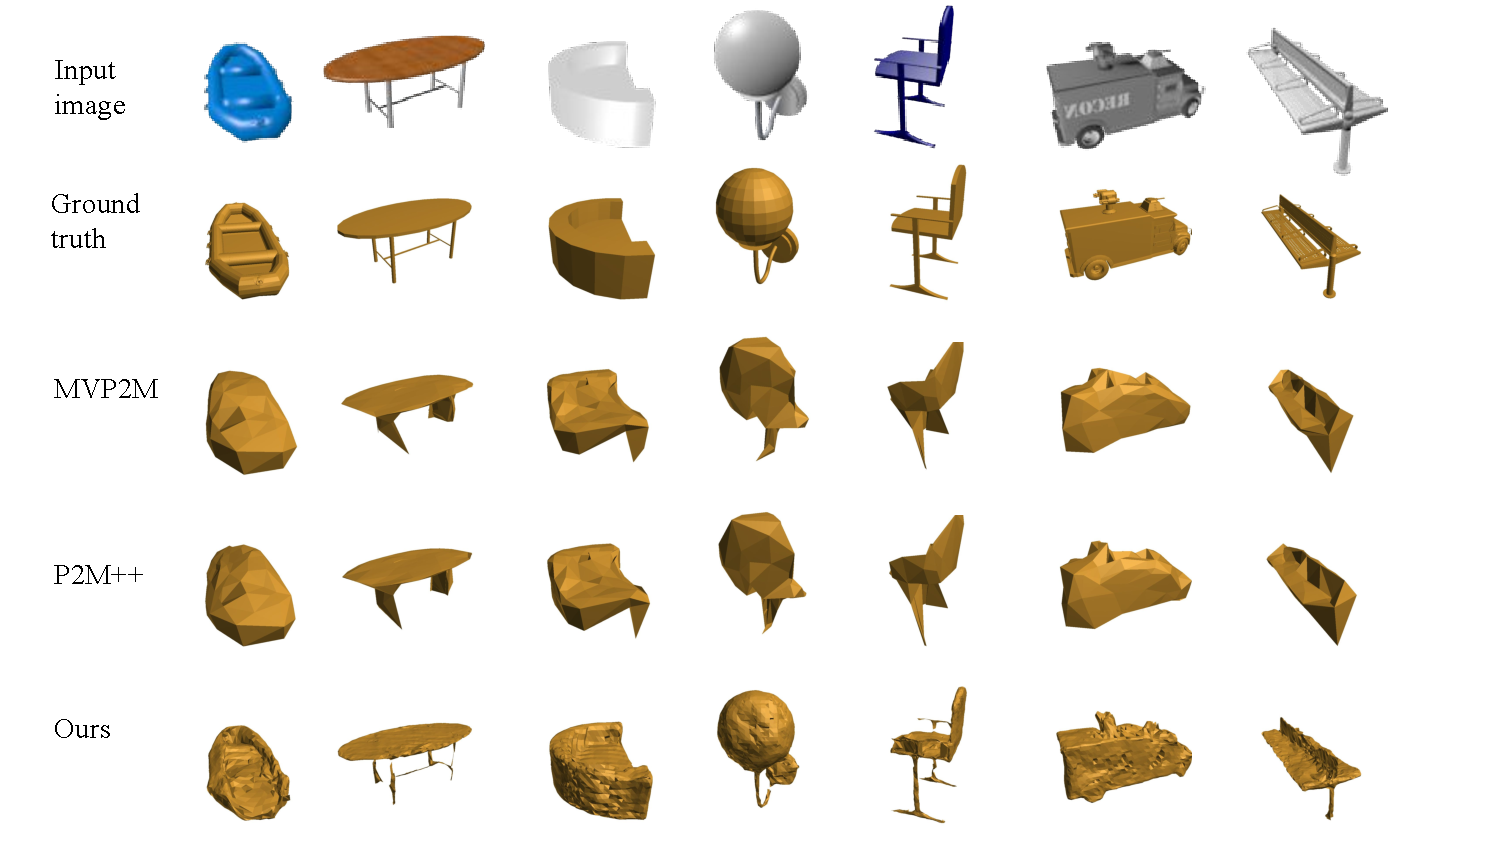
\includegraphics[width=\linewidth]{imgs/qualitative_evaluation.pdf}
\end{center}
\caption{
    \textbf{Qualitative evaluation} on ShapeNet dataset. \textbf{From top to bottom}: one of the input images, ground truth mesh, multi-view extended Pixel2Mesh, Pixel2Mesh++, and ours.
    Our predictions are closer to the actual shape, especially for the objects with more complex topology.}

    % Two of three input images used by all the systems are shown along with a pair of camera views of the predictions.
    % The quality of shapes generated by our method is consistently better.
    % Note that in the last input of category \emph{Watercraft} the baselines generate shapes closer to \emph{Car} while our predictions are much closer to the actual shape.
% }
\label{fig:qualitative_evaluation}
\end{figure*}

\subsection{Experimental Setup}
\label{subsec:experimental_setup}

\paragraph{Comparisons}
We evaluate the proposed method against various multi-view shape generation methods.
The state-of-the-art method is Pixel2Mesh++~\cite{wen2019pixel2mesh++} (referred as \emph{P2M++}). \cite{wen2019pixel2mesh++} also provide a baseline by directly extending Pixel2Mesh~\cite{wang2018pixel2mesh} to operate on multi-view images (referred as \emph{MVP2M}) using their statistical feature pooling method to aggregate features from multiple color images.
% This implementation is closer to \emph{Ours-P2M} system design in that it predicts the output mesh by series for GCN deformations
% starting from an initial ellipsoid without having a fairly accurate initial object mesh.
% Also, \emph{Ours-P2M} uses the same architecture for the mesh deformations as \emph{MVP2M}. Hence, the changes in performance can be directly attributed to our depth based features, added geometric constraints and attentive feature pooling.
Results from additional multi-view shape generation baselines 3D-R2N2~\cite{3dr2n2} and LSM~\cite{kar2017lsm} are also reported.

\paragraph{Dataset}\vspace{-4mm}
We evaluate our method against the state-of-the-art methods on the dataset from~\cite{3dr2n2}
which is a subset of ShapeNet~\cite{chang2015shapenet} and has been widely used by recent 3D shape generation methods.
It contains 50K 3D CAD models from 13 categories.
Each model is rendered with a transparent background from 24 randomly chosen camera viewpoints to obtain color images.
The corresponding camera intrinsics and extrinsics are provided in the dataset.
Since the dataset does not contain depth images, we render them using a custom depth renderer at the same viewpoints as the color images and with the same camera intrinsics.
We follow the training/testing/validation split of~\cite{gkioxari2019meshrcnn}.

\paragraph{Implementation}\vspace{-4mm}
% We train the proposed model using the same settings as Pixel2Mesh++ and MVP2M for fair comparison.
% The same 3 views from each model are used as input and the images are resized to a resolution of 224$\times$224 for feature extraction/depth prediction.
For the depth prediction module, we follow the original MVSNet~\cite{yao2018mvsnet} implementation.
The output depth dimensions reduces by a factor of 4 to 56$\times$56 from the 224$\times$224 input image.
The number of depth hypotheses is chosen as 48 which offers a balance between accuracy and running/training time efficiency.
These depth hypotheses represent values from $0.1$ m to $1.3$ m at an interval of $25$ mm.
These values were chosen based on the range of depths present in the dataset.
% The final cost volume is of dimensions 56$\times$56$\times$48 which is regularized using a 3D convolutional network.

The hierarchical features obtained from "Contrastive Depth Features Extractor" are of total 4800 dimensions for each view.
The aggregated multi-view features are compressed to 480 dimensional after applying attentive feature pooling.
5 attention heads are used for merging multi-view features.
The loss function weights are set as $\lambda_{\text{chamfer}}=1$, $\lambda_{\text{normal}}=1.6\times10^{-4}$, $\lambda_{\text{depth}}=0.1$, $\lambda_{\text{contrastive}}=0.001$ and $\lambda_{\text{voxel}}=1$.
Two settings of $\lambda_{\text{edge}}$ were used, $\lambda_{\text{edge}}=0$ (referred as \emph{Best}) which gives better quantitative results and $\lambda_{\text{edge}}=0.2$ (referred as \emph{Pretty}) which gives better qualitative results.

% Ours models are implemented in PyTorch deep learning framework using open-source Pixel2Mesh/Mesh R-CNN implementation.

% \siyu{Unlike~\cite{yao2018mvsnet}, we do not apply input image view selection and use the input views from~\cite{3dr2n2,wen2019pixel2mesh++} for fair comparison.
% }

\paragraph{Training and Runtime}\vspace{-4mm}
The network is optimized using Adam optimizer with a learning rate of $10^{-4}$.
The training is done on 5 Nvidia RTX-2080 GPUs with effective batch size 5.
% The number of GPUs and batch size were chosen in order to maximize training speed while staying within the GPU memory limit.
The depth prediction network (MVSNet) is trained independently for 30 epochs.
Then the whole system is trained for another 40 epochs with the weights of the MVSNet frozen.
Our system is implemented in PyTorch deep learning framework and it takes around 60 hours for training.

% The initial learning rate is set to 1e-4 which is reduced to 1e-5 after 30 epochs and 1e-6 after 45 epochs.
% \emph{Ours-P2M} takes around 100 hours to train while \emph{Ours-MRCNN} takes around 50 hours.
% This training time is similar to Pixel2Mesh++.

\paragraph{Evaluation Metric}\vspace{-4mm}
Following~\cite{wang2018pixel2mesh, wen2019pixel2mesh++}, we use F1-score as our evaluation metric.
The F1-score is the harmonic mean of precision and recall where the precision/recall are calculated by finding the percentage of points in the predicted/ground truth that can find a nearest neighbor from the other within a threshold.
We provide evaluations with two threshold values: $\tau$ and $2\tau$ where $\tau=10^{-4}$  m$^2$.
% (in terms of squared Euclidean distance).
% The output meshes can vary in number of vertices but are re-sampled to 6466 points before evaluating the F1-score~\cite{wang2018pixel2mesh, wen2019pixel2mesh++}. \rakesh{might not be true}

\subsection{Comparison with previous Multi-view Shape Generation Methods}
We quantitatively compare our method against previous works for multi-view shape generation in~\tableref{baseline_comparison} and show the effectiveness of our methods in improving the shape quality. Our method outperforms the state-of-the-art method  Pixel2Mesh++~\cite{wen2019pixel2mesh++} with
a decrease in chamfer distance to ground truth by 34\% and 15\% increase in F1-score at threshold $\tau$.
Note that in~\tableref{baseline_comparison} the same model is trained for all the categories but accuracy on individual categories as well as average over the categories are evaluated.
We provide the chamfer distances in the appendix.
\begin{table}[ht]
\begin{center}
\resizebox{\linewidth}{!}{
\begin{tabular}{|c|cccccc|cccccc|}
    \hline
    \multirow{3}{*}{Category}&
    \multicolumn{6}{c|}{F-score ($\tau$) $\uparrow$}&
    \multicolumn{6}{c|}{F-score ($2\tau$) $\uparrow$}\\
    & \multirow{2}{*}{3D-R2N2}  & \multirow{2}{*}{LSM}  & \multirow{2}{*}{MVP2M}    & \multirow{2}{*}{P2M++} & Ours & \bf{Ours}
    & \multirow{2}{*}{3D-R2N2}  & \multirow{2}{*}{LSM}  & \multirow{2}{*}{MVP2M}    & \multirow{2}{*}{P2M++} & Ours & \bf{Ours} \\
    &                           &                       &                           &                        & (pretty) & \bf{(best)} &
                                &                       &                           &                        & (pretty) & \bf{(best)} \\
    \hline
    Couch       & 45.47 & 43.02 & 53.17 & 57.56 & 71.63 & \bf{73.63}    & 59.97 & 55.49 & 73.24 & 75.33 & 85.28 & \bf{88.24} \\
    Cabinet     & 54.08 & 50.80 & 56.85 & 65.72 & 75.91 & \bf{76.39}    & 64.42 & 60.72 & 76.58 & 81.57 & 87.61 & \bf{88.84} \\
    Bench       & 44.56 & 49.33 & 60.37 & 66.24 & 81.11 & \bf{83.76}    & 62.47 & 65.92 & 75.69 & 79.67 & 90.56 & \bf{92.57} \\
    Chair       & 37.62 & 48.55 & 54.19 & 62.05 & 77.63 & \bf{78.69}    & 54.26 & 64.95 & 72.36 & 77.68 & 88.24 & \bf{90.02} \\
    Monitor     & 36.33 & 43.65 & 53.41 & 60.00 & 74.14 & \bf{76.64}    & 48.65 & 56.33 & 70.63 & 75.42 & 86.04 & \bf{88.89} \\
    Firearm     & 55.72 & 56.14 & 79.67 & 80.74 & 92.92 & \bf{94.32}    & 76.79 & 73.89 & 89.08 & 89.29 & 96.81 & \bf{97.67} \\
    Speaker     & 41.48 & 45.21 & 48.90 & 54.88 & 66.02 & \bf{67.83}    & 52.29 & 56.65 & 68.29 & 71.46 & 79.76 & \bf{82.34} \\
    Lamp        & 32.25 & 45.58 & 50.82 & 62.56 & 72.47 & \bf{75.93}    & 49.38 & 64.76 & 65.72 & 74.00 & 82.00 & \bf{85.33} \\
    Cellphone   & 58.09 & 60.11 & 66.07 & 74.36 & 85.57 & \bf{86.45}    & 69.66 & 71.39 & 82.31 & 86.16 & 93.40 & \bf{94.28} \\
    Plane       & 47.81 & 55.60 & 75.16 & 76.79 & 89.23 & \bf{92.13}    & 70.49 & 76.39 & 86.38 & 86.62 & 94.65 & \bf{96.57} \\
    Table       & 48.78 & 48.61 & 65.95 & 71.89 & 82.37 & \bf{83.68}    & 62.67 & 62.22 & 79.96 & 84.19 & 90.24 & \bf{91.97} \\
    Car         & 59.86 & 51.91 & 67.27 & 68.45 & 77.01 & \bf{80.43}    & 78.31 & 68.20 & 84.64 & 85.19 & 88.99 & \bf{92.33} \\
    Watercraft  & 40.72 & 47.96 & 61.85 & 62.99 & 75.52 & \bf{80.48}    & 63.59 & 66.95 & 77.49 & 77.32 & 86.77 & \bf{90.35} \\
    \hline
    Mean        & 46.37 & 49.73 & 61.05 & 66.48 & 78.58 & \bf{80.80}    & 62.53 & 64.91 & 77.10 & 80.30 & 88.49 & \bf{90.72} \\
    \hline
\end{tabular}}
\end{center}
\vspace{-4mm}
\caption{
    \textbf{Qualitative comparison} against state-of-the-art multi-view shape generation methods. We report F-score on each semantic category along with the mean over all categories using two thresholds $\tau$ and $2\tau$ for nearest neighbor match where ${\tau}$=$10^{-4}$ m$^2$.
}
\label{table:baseline_comparison}
\end{table}



We also provide visual results for qualitative assessment of the generated shapes by our \emph{Pretty} model in~\figref{qualitative_evaluation} which shows that it is able to more accurately predict topologically diverse shapes.

% ~\tableref{baseline_comparison} show the ablation study
% performed to quantify the improvements from different aspects of our methods.
% Our methods outperform all the baselines in all the semantic categories.
% \figref{qualitative_evaluation} shows the qualitative comparison between the shapes generated by the different methods.
% The baseline methods suffer from various artifacts and discontinuities while ours generate shapes with higher fidelity.

\subsection{Ablation studies}
% Extensive ablation studies are performed to quantify the contributions of each component.
% The "stats pooling" baseline is obtained by replacing the attention-based feature pooling with statistical features from Pixel2Mesh++.
% Similarly, "simple attention" baseline is obtained by replacing our feature pooling with feature fusion technique proposed in~\cite{hu2019randla,yang2020robust} where the pooled features are weighted sum of the multi-view features.
% We can see that our rendered depth loss, contrastive depth input and attention-based feature pooling individually improve the accuracy of the predicted mesh.

% \begin{table}[ht]
% \begin{center}
% \resizebox{\linewidth}{!}{
% \begin{tabular}{|c|c|c|c|c|c|c|}
%     \hline
%     Metric & Ours-P2M & - rendered depth loss & - contrastive depth & stats pooling & simple attention & GT-depth \\
%     \hline
%     F1-$\tau$ & TBD & TBD & TBD & TBD & TBD & \textbf{TBD} \\
%     F1-$2\tau$ & TBD & TBD & TBD & TBD & TBD & \textbf{TBD} \\
%     % Chamfer distance (mm) & 0.30 & 0.33 & 0.33 & 0.325 & 0.30 & \textbf{0.18} \\
%     \hline
% \end{tabular}}
% \end{center}
% \caption{
%     Ablation Study. ${\tau}$=$10^{-4}$ m$^2$
% }
% \label{table:ablation_study_p2m}
% \end{table}

\begin{table}[ht]
% \captionsetup{font=footnotesize,labelfont=footnotesize}
\begin{center}
\footnotesize
\begin{tabular}{ l c c }
\toprule[1pt]
 &F1-$\tau$ &F1-2$\tau$   \\ \hline
(1) Naive multi-view Mesh R-CNN \qquad \qquad  \qquad  \qquad  \qquad & 72.74 & 84.99 \\
(2) + Multi-view voxel grid prediction & 76.97 & 88.24 \\
(3) + Contrastive depth input             & 79.63 & 90.10 \\
(4) + Multi-head attention pooling   & 79.82    & 90.18  \\
(5) \bf{+ Contrastive depth loss (final model)}  & \textbf{80.80} & \textbf{90.72}\\
% (6) Baseline + rendered vs GT depth loss    & 80.35 & 90.55 \\
% (7) Baseline + rendered vs predicted depth loss + rendered vs GT depth loss    & 80.45 & 90.56 \\
% (8) Baseline with simple attention          & 80.03 & 90.21 \\
(6) Using GT depth (final model)                 & \textbf{84.58} & \textbf{92.86} \\
% (10) Sphere initialization                  & 73.78 & 85.49 \\
\bottomrule[1pt]
\end{tabular}
\end{center}
\vspace{-4mm}
\caption{
    \textbf{Comparison of shape generation accuracy with different settings} of additional contrastive depth losses, multi-view feature pooling.
    The Baseline framework uses multi-head attention mechanism without any contrastive depth losses.
    \siyu{Remove (2) Multi-head attention pooling and (6) Using GT depth (final model). Both statistics seem to be irrelevant to the paper.}
}
\label{table:ablation_study}
\end{table}

% \begin{table}[t]
% % \captionsetup{font=footnotesize,labelfont=footnotesize}
% \begin{center}
% \footnotesize
% \begin{tabular}{ l c c }
% \toprule[1pt]
%  &F1-$\tau$ &F1-2$\tau$ \\ \hline
% With Perceptual Feature Loss \qquad \qquad  \qquad  \qquad  \qquad  & 74.87 & 86.92 \\
% Without Perceptual Feature Loss & 75.30 & 87.12 \\
% \bottomrule[1pt]
% \end{tabular}
% \end{center}
% \caption{Comparisons of different contrastive depth formulations, where \emph{Pred} indicates predicted depth map from MVSNet, \emph{Rend} indicates rendered depth map from deformed mesh model, $\ominus$ means element-wise minus, $\otimes$ means concatenation. In 1 and 2 concatenation and difference of the depths are fed to VGG feature extractor while in 3 and 4 concatenation and difference of the VGG features from the depths is used for mesh refinement \rakesh{Note: These results will be updated with the results from our final architecture}}
% \label{table:perceptual_loss}
% \end{table}


\paragraph{Accuracy with different settings}\vspace{-4mm}
\tableref{ablation_study} shows the contribution of different components towards the final accuracy. Naively extending the single-view Mesh R-CNN~\cite{gkioxari2019meshrcnn} to multiple views using statistical feature pooling~\cite{wen2019pixel2mesh++} for mesh refinement (row 1) gives an F1-score of 72.74\% for threshold $\tau$ which is 6.26\% improvement over Pixel2Mesh++.
We further extend the above method with our probabilistic multi-view voxel grid prediction in row 2 and get a 4.23\% improvement.

In row 3 of~\tableref{ablation_study} we use our contrastive depth features instead of RGB features for mesh refinement and get 2.7\% improvement.
We then replace the statistical feature pooling with the proposed attention method and get 0.19\% improvement.
The improvement is not significant on our final architecture but we found the multi-head attention to perform better on more light-weight architectures.
We also evaluate the effect of using additional regularization from contrastive depth losses: rendered depth vs predicted depth in the 5th rows of which improves the score by 0.98\%.
In row 6 we use ground truth instead of predicted depths on our final model which gives the upper bound on our mesh prediction accuracy in relation to the depth prediction accuracy as 84.58\%.

\begin{table}[ht]
% \captionsetup{font=footnotesize,labelfont=footnotesize}
\begin{center}
\footnotesize
\begin{tabular}{ l c c }
\toprule[1pt]
 &F1-$\tau$ &F1-2$\tau$   \\ \hline
(1) P2M++ & 66.48 & 80.30 \\
(2) Sphere initialization & 73.78 & 85.49 \\
(3) Back-projected predicted depth initialization & 75.62 & 86.53 \\
% (3) + Multi-view voxel grid prediction & 76.97 & 88.24 \\
% this does not use contrastive depth features/loss and attention pooling, so is inconsistent with others
(4) \bf{Proposed model}  & \textbf{80.80} & \textbf{90.72}\\
\bottomrule[1pt]
\end{tabular}
\end{center}
\vspace{-4mm}
\caption{
    \textbf{Comparison of shape generation accuracy with different initial shapes}: sphere, back-projected depth and the proposed model (CNN-based multi-view voxel grid prediction)}
\label{table:initial_shape}
\end{table}


\paragraph{Initial Shape}\vspace{-4mm}
\tableref{initial_shape} shows the F1-scores when using different methods for generating initial shapes for GCN refinement.
All the methods (except P2M++) use contrastive depth features and loss along with attention-based feature pooling.
When a unit level-4 ico-sphere is used as the initial shape (row 2), the score is F1-$\tau$ 73.78\%.
Using back-projected predicted depth maps as initial shape (row 3), the scores increases to 75.62\%.
Here, the back-projected points are transformed to 48 $\times$ 48 $\times$ 48 voxel grid.
This can be done differentiably and efficiently using GPU-based chamfer distance calculation to determine the occupancy of each voxel.
The proposed model which uses CNN-based voxel grid prediction (row 4) has the highest score of 80.8\%.
The difference in score when using back-projected depth vs CNN predicted shape is due to the incomplete shapes the predicted depth give due to occlusion along with depth error due to arbitrary baseline between input images which is challenging to MVSNet depth predictor.

\paragraph{Contrastive Depth Feature Extraction}\vspace{-4mm}
We evaluate several methods for contrastive feature extraction (\subsecref{contrastive_depth_feature_extraction}). These methods are
1) \emph{Input Concatenation}: using the concatenated rendered and predicted depth maps as input to the CNN feature extractor,
2) \emph{Input Difference}: using the difference of the two depth maps as input to CNN,
3) \emph{Feature Concatenation}: concatenating features from rendered and predicted depths extracted by shared CNN,
4) \emph{Feature Difference}: using difference of the features from the two depth maps extracted by shared CNN, and
5) \emph{Predicted depth only}: using the CNN features from the predicted depths only.
6) \emph{Rendered depth only}: using the CNN features from the rendered depths only.
The quantitative results are summarized in Table~\ref{table:contrastive_feature_extraction} and shows that \emph{Input Concatenation} method produces better results than other formulations.
% remains more details depth information and our Contrastive Depth Feature Extraction is able to encode the difference between the predicted depth map and rendered depth map from each deformation stage.

\begin{table}[ht]
% \captionsetup{font=footnotesize,labelfont=footnotesize}
\begin{center}
\footnotesize
\begin{tabular}{ l c c }
\toprule[1pt]
 &F1-$\tau$ &F1-2$\tau$ \\ \hline
(1) Input Concatenation \qquad \qquad  \qquad  \qquad  \qquad  & \textbf{80.80} & \textbf{90.72} \\
(2) Input Difference & 80.41 & 90.54 \\
(3) Feature Concatenation   & 80.45 & 90.54 \\
(4) Feature Difference & 80.30 & 90.40 \\
(5) Predicted Depth only & 79.40 & 89.95 \\
(6) Rendered Depth only & 78.20 & 88.90 \\
\bottomrule[1pt]
\end{tabular}
\end{center}
\vspace{-4mm}
\caption{\textbf{Comparisons of different contrastive depth formulations}. In 1st and 2nd rows, concatenation and difference of the rendered and predicted depths are fed to VGG feature extractor while in 3rd and 4th rows, concatenation and difference of the VGG features from the depths is used for mesh refinement. 5 uses VGG features from predicted depths only while 6 uses VGG features from rendered depths only. \siyu{``Input Concatenation'' and ``Input Difference'' are hard to understand. Change them to another expression, such as ``Depth image concatenation''.}}
\label{table:contrastive_feature_extraction}
\end{table}




% using the difference
% Instead of using contrastive depth input i.e. concatenated predicted and rendered depths
% (refer to~\figref{system_architecture})
% we directly use a single channeled predicted depth as input. Column 4 of
% \tableref{ablation_study} and \tableref{ablation_study_mrcnn} show the results of these experiments.

% % \begin{table}[ht]
% \begin{center}
% \footnotesize
% \begin{tabular}{c | c c c c c c}
%     \hline
%     Metric & RGB-Ours & Depth-Ours & RGBD-Ours & RGB 1-view & Depth 1-view & RGBD 1-view \\
%     \hline
%     F1-$\tau$   & 31.27 & 30.30 & 31.61 & 25.19 & 23.78 & 26.06 \\
%     F1-$2\tau$  & 44.46 & 43.16 & 44.86 & 36.75 & 35.14 & 37.74 \\
%     \hline
% \end{tabular}
% \end{center}
% \caption{
%     Accuracy of predicted voxel of individual views against probabilistically merged multi-view voxel grids, where the first three columns indicate the accuracy of multi-view voxel generations while the last three columns show single-view. The voxel branch was trained separately without the mesh refinement. Evaluation is conducted after cubify and the depth maps are generated from MVSNet.
% }
% \label{table:multiview_voxel_accuracy}
% \end{table}
\begin{table}[ht]
\noindent \scriptsize \footnotesize
\begin{minipage}[t]{0.5\textwidth}
\centering
\begin{tabular}{c | c c}
    \hline
    Metric      & Single-view & Multi-view \\
    \hline
    F1-$\tau$   & 25.19 & 31.27 \\
    F1-$2\tau$  & 36.75 & 44.46 \\
    \hline
\end{tabular}
\caption{
    \textbf{Accuracy of predicted voxel grids} from single-view prediction compared against the proposed probabilistically merged multi-view voxel grids. The voxel branch was trained separately without the mesh refinement and evaluation was performed on the cubified voxel grids. We use three views for probabilistic grid merging.
}
\label{table:multiview_voxel_accuracy}
\end{minipage}
\hspace{0.1cm}
\noindent \scriptsize \footnotesize
\begin{minipage}[t]{0.5\textwidth}
\centering
\begin{tabular}{c | c c c c}
    \hline
    Metric & Cubified & Stage-1 & Stage-2 & Stage-3 \\
    \hline
    F1-$\tau$   & 31.48 & 76.78 & 79.88 & 80.80  \\
    F1-$2\tau$  & 44.40 & 88.32 & 90.19 & 90.72  \\
    \hline
\end{tabular}
\caption{
    \textbf{Accuracy of the refined meshes at different GCN stages}. 1, 2 and 3 indicate the performance at the corresponding graph convolution blocks while \emph{Cubified} is for the cubified voxel grids used as input for the first GCN block. All the stages, including the voxel prediction, were trained jointly and hence the accuracy of voxel predictions varies from that in~\tableref{multiview_voxel_accuracy}.
}
\label{table:gcn_stages}
\end{minipage}
\end{table}



% \paragraph{Different Input Modalities}
% We analyze the accuracy of using different input modalities (RGB vs Depth vs RGB-D) for the voxel branch and mesh branch (GCN refinement) in~\tableref{input_modality_accuracy}.

% \begin{table}[ht]
\begin{center}
\footnotesize
\begin{tabular}{c c | c c}
\toprule[1pt]
    Voxel branch    & Mesh branch   & F1-$\tau$         & F1-$2\tau$ \\ \hline
    RGB             & RGB           & 79.66             & 89.98 \\
    Depth           & Depth         & 77.07             & 88.20 \\
    RGB-D           & RGB           & 78.42             & 89.32 \\
    RGB             & RGB-D         & \textbf{80.80}    & \textbf{90.55} \\
    % RGB-D         & RGBD-D        & \textbf{81.15}    & \textbf{90.92}
\bottomrule[1pt]
\end{tabular}
\end{center}
\caption{
    Accuracy with different input modalities of voxel and mesh.
    % \rakesh{More extensive combinations of input modalities can be performed if needed}
    % Using RGB-D for both voxel and mesh branch gave the best results with the most recent architecture
    % but all the other ablation study experiments were performed with RGB+RGB-D, so we are not reporting RGBD+RGBD to avoid confusion
}
\label{table:input_modality_accuracy}
\end{table}



\paragraph{Number of Views}\vspace{-4mm}
We test the performance of our framework with respect to the number of views.
\tableref{number_of_input_views} shows that the accuracy of our method increases as we increase the number of input views for training.
These experiments also validate that the attention-based feature pooling can efficiently encode features from different views to take advantage of larger number of views.

\tableref{number_of_test_views} shows the results when using different number of views during testing on our model trained with 3 views
which indicates that increasing the number of views during testing does not improve the accuracy while decreasing the number of views can cause a significant drop in accuracy.
% The accuracy is very close to the corresponding models trained with higher number of views indicating our model can learn with fewer number of views and generalize to a larger number.
% -> \rakesh{this conclusion is not true, training with larger number of views gets significantly better performance}
\begin{table}[ht]
\noindent \scriptsize \footnotesize
\begin{minipage}[t]{0.5\textwidth}
\centering
\begin{tabular}{ l | c c c c c }
    \hline
    Metric & 2 & 3 & 4 & 5 & 6\\
    \hline
    F1-$\tau$  & 73.60 & 80.80 & 82.61 & 83.76 & 84.25 \\
    F1-$2\tau$ & 85.80 & 90.72 & 91.78 & 92.73 & 93.14 \\
    \hline
\end{tabular}
\caption{
    \textbf{Accuracy w.r.t the number of views during training}.
    The evaluation was performed on the same number of views as training.
    % The evaluation was performed on the same number of views (3 views) for a fair comparison. \rakesh{Not true}
}
\label{table:number_of_input_views}
\end{minipage}
\hspace{0.1cm}
\noindent \scriptsize \footnotesize
\begin{minipage}[t]{0.5\textwidth}
\centering
\begin{tabular}{ l | c c c c c }
    \hline
    Metric & 2 & 3 & 4 & 5 & 6 \\
    \hline
    F1-$\tau$   & 72.46 & 80.80 & 80.98 & 80.94 & 80.85 \\
    F1-$2\tau$  & 84.49 & 90.72 & 91.03 & 91.16 & 91.20 \\
    \hline
\end{tabular}
\caption{
    \textbf{Accuracy w.r.t the number of views during testing}.
    The same model trained with 3 views was used in all of the cases.
}
\label{table:number_of_test_views}
\end{minipage}
\vspace{-4mm}
\end{table}
\vspace{-4mm}


%%%%%%%%% Conclusion
\section{Conclusion}

We propose a neural network based solution to predict 3D triangle mesh models of objects from images taken from multiple views.
First, we propose a multi-view voxel grid prediction module which probabilistically merges voxel grids predicted from individual input views.
We then cubify the merged voxel grid to triangle mesh and apply graph convolutional networks for further refining the mesh.
The features for the mesh vertices are extracted from contrastive depth input consisting of rendered depths at each refinement stage along with the predicted depths.
The proposed mesh reconstruction method outperforms existing methods with a large margin and is capable of reconstructing objects with more complex topologies.
% Our system exploits the recent developments on multi-view depth prediction to inform the mesh generation process and obtains state-of-the-art performance.
% We also present a novel method for aggregating features from multiple images which takes into account the importance of each view for predicting different parts of the objects.



{\small
\bibliographystyle{ieee_fullname}
\bibliography{egbib}
}

\end{document}
